\documentclass[a4paper]{article}

\usepackage[english]{babel}
\usepackage[utf8]{inputenc}
\usepackage{amsmath}
\usepackage{graphicx}
\usepackage[colorinlistoftodos]{todonotes}


\title{Biogears in Anesthesia Screen Based Simulation}

\author{
  Xiao Han\\
  \and Liewei Ke
  \and Guan Wang
  \and Mclvor William
}

\date{\today}

\begin{document}
\maketitle

\begin{abstract}
The delivery of good medical care concerns patients as well as medical professionals. In terms of medical training, mannequins used to be orthodox way to train and demonstrate medical skills for students. Nowadays, schools and institutions are adopting more and more high-tech involved methodologies such as Simulation-Based medical education, Virtual Reality in order to provide students with immersive and realistic experience of medical training. In Simulation-Based medical education particularly, whether the models of physiology incidents or responses are accurate or not will directly affect the credibility of the simulation. In this paper, we will give insights into the physiology simulation and compare the current physiology engine Biogears. We will evaluation its function by comparing with simulation provided by CAE Muse system. In the end, we will conclude on the performance of Biogears on key points such as authenticity, stability as well as commenting on its limitations.
\end{abstract}

\section{Current physiologic engines and BioGears}
There are a lot of physiologic engines or simulation softwares out there that provides ability to simulate sophisticated body systems. Some of them are licensed so medical schools or institutions will have to buy them for usage. For example, CAE is a simulation company that provides simulation for aviation, security(defense) and healthcare. Their main product for medical simulation is Muse. Must provides several simulation scenarios where patients come with different conditions.

Biogears is an open-source physiology engine that provides accurate as well as consistent physiologic simulation of human bodies. It contains models that mimic human systems as circuits and substance in physiology for real-time input. It can be used as standalone application where physicians could use integrated GUI to simulate customized scenarios or integrated with mannequins, sensors or interfaces that utilize the engine to output consistently.

To thoroughly evaluate Biogears simulation, we repeatedly conducted several experiments on normal patients and calculate key variables within the patients. We evaluate engine stability by calculating the mean squared error of several vital signs. We evaluate engine authenticity by comparing with CAE simulation result and consulting with real doctors and physicians.  



\section{Show equivalence to current training methods}

- how to show current training methods

\subsection{Current training methods}
\subsection{Why using screen based simulation is equivalent to current training methods}

\section{Show physiologically appropriate, responses to key events}

The reason why physicians don't buy into simulation-based software is due to the fundamental distrust in the models simulation software utilized to generate all the signals and data. And yet, there is no uniformly consented algorithms to describe the complicated nature of human bodies. Thus, the most reliable way to evaluate whether a simulation is fit for real scenario operations is to compare them with the common sense of physicians and doctors. For example, one of the most common thoughts of physicians about the authenticity of scenarios generated by simulation is to see the heart rate of patient when the patient is given different dosage of morphine. If you inject a small dosage of morphine it should somehow make the patient calm down and reduce the heart rate but if you inject more morphine than you should, the drug may be likely to kill a patient. 

Inspired by the previous work from this paper \cite{measure_repeatability}, we think the quality of a simulation system will also be determined by the stability of experiments under the same or similar circumstances. After consulting with physicians from UPMC and Biogears team, we enumerate several representative experiments and ran both Biogears and CAE simulation on them. Later we presented the result in graphs and tables for visuality.

\subsection{Bleeding Out Scenarios}

Bleeding patients are often seen in trauma and emergency rooms. The cause of this symptom varies. Car accident, Blood vessel abnormalities, blood disorders, tumors, to name a few. We believe that to see how simulation engine reacts to a patient who is suffering from bleeding would be a good way to see how it models human bodies change as time goes by.

To run this experiment on Biogears, we tested it using built-in GUI of Biogears that provides dozens of substances simulation.  

\begin{figure}
  \centering
  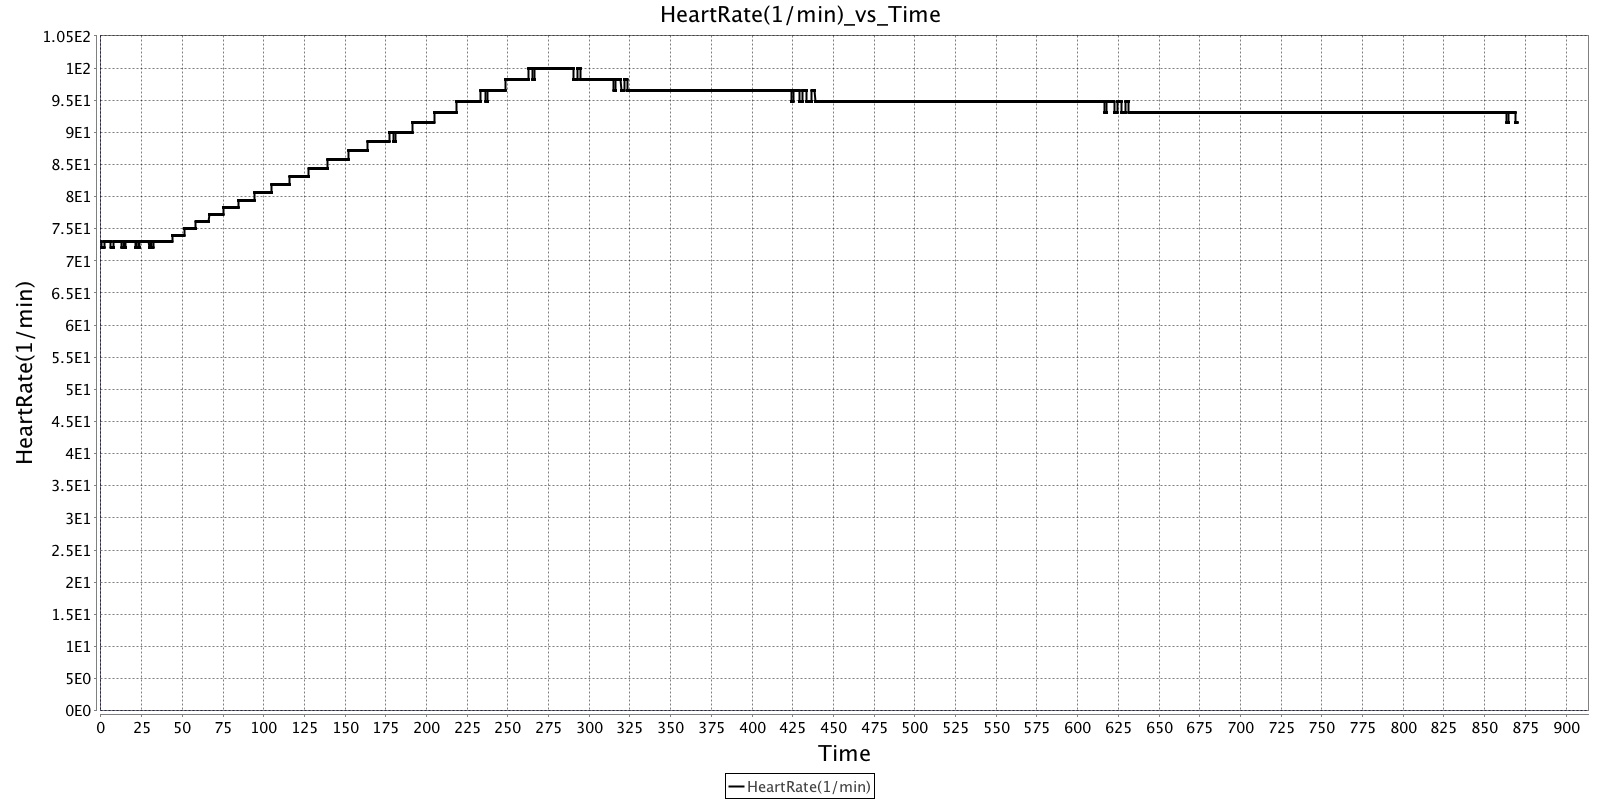
\includegraphics[width=10cm]{bleeding_out_HeartRate_vs_Time.jpg}
  \caption{heart rate changes when patient bleeds out in Biogears simulation}
  \label{fig:patient bleeding}
\end{figure}

\begin{figure}
  \centering
  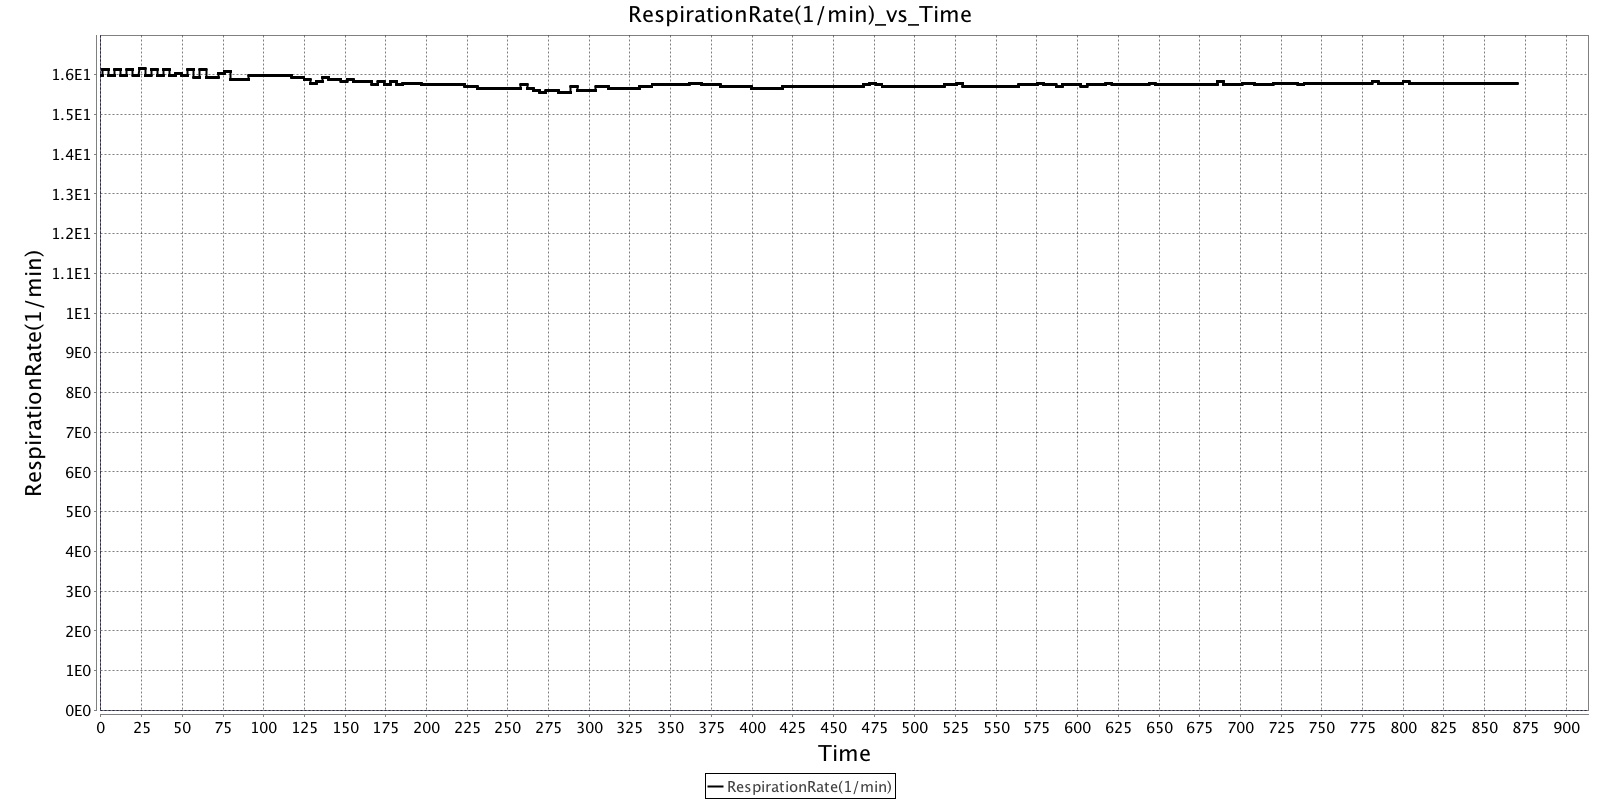
\includegraphics[width=10cm]{bleeding_out_RespirationRate_vs_Time.jpg}
  \caption{heart rate changes when patient bleeds out in Biogears simulation}
  \label{fig:patient bleeding}
\end{figure}

In reality, it is not the case that patient could live with continuous hemorrhage: The heart rate of patient will increase because with blood loss there is not enough oxygen so his/her heart has to pump faster and absorb more oxygen. His respiratory rate will rise. But after a while, when he/she eventually loses 


- bleeding out scenarios, multiple experiments, (mean, root mean squared error, median performance error data recorded)
- oxygen desaturation (same as aboved)

- patient stop breathing for 30 seconds, 2 mins and recover

- (optional) compare with another dataset asac dataset

- simulate with propofal(200mg), morphine so4(20mg), rocuromium(50mg), succinocloon(100mg), room air(170/70kg)

\subsection{Physical experiments}
\subsection{Other simulators}

\section{Enumerate limits and future work}
\subsection{Limits of screen based simulation}
\subsection{Future work}

\begin{thebibliography}{1}

  \bibitem{measure_repeatability} Cumin, David, Charlotte Chen, and Alan F. Merry. "Measuring the repeatability of simulated physiology in simulators." Simulation in Healthcare 10.6 (2015): 336-344.

  \bibitem{impj}  

  \bibitem{norman} 

  \bibitem{fo} 

  \end{thebibliography}
\end{document}